\documentclass[11pt,a4paper]{article}

% ─── Packages ────────────────────────────────────────────────────────────────
\usepackage[T1]{fontenc}
\usepackage[utf8]{inputenc}
\usepackage{lmodern}
\usepackage[a4paper,margin=2.5cm]{geometry}
\usepackage{amsmath,amssymb}
\usepackage{graphicx}
\usepackage{booktabs}
\usepackage{caption}
\usepackage{subcaption}
\usepackage{xcolor}
\usepackage{hyperref}
\usepackage{listings}
\usepackage{tikz}
\usetikzlibrary{shapes.geometric, arrows.meta, positioning, fit, backgrounds}
\usepackage{microtype}
\usepackage{authblk}
\usepackage{siunitx}
\usepackage{lineno}
% \linenumbers  % uncomment for submission

\hypersetup{
    colorlinks=true,
    linkcolor=blue!50!black,
    urlcolor=blue!50!black,
    citecolor=blue!50!black
}

\lstset{
  basicstyle=\ttfamily\small,
  breaklines=true,
  frame=single,
  framesep=4pt,
  rulecolor=\color{gray!30},
  backgroundcolor=\color{gray!5}
}

% ─── Title ───────────────────────────────────────────────────────────────────
\title{\textbf{Interpretable Sentinel-2 Turbidity Mapping with Ensemble Symbolic Regression}\\[0.4em]
\large A Reproducible Visual-Programming Pipeline for the Lower Seine}

\author[1]{Nicolas Priniotakis\thanks{Corresponding author: \texttt{nicolas.priniotakis@unilasalle.fr}}}
\affil[1]{UniLaSalle}

\date{\today}

\begin{document}
\maketitle

% ─── Abstract ────────────────────────────────────────────────────────────────
\begin{abstract}
We present a \textbf{proof-of-concept} pipeline for estimating water turbidity (NTU) from Sentinel-2 surface reflectance using an ensemble of genetic-programming (GP) symbolic regressors. The pipeline is built as a visual node graph inside the open-source environment \textbf{VNStudio}, exposing every parameter on a connectable node and serializing the entire experiment to a single JSON file. Training uses 563 satellite--station matchups assembled from the French Hub'Eau Naïades network for the lower Seine basin (2017--2025); stratified subsampling of the Clear (<5\,NTU) class is required to prevent the GP search from collapsing to a near-constant predictor. Ten independent GP runs aggregate into a mean turbidity map ($\mu$) and a per-pixel ensemble-spread map ($\sigma$). Applied to a 10\,m July 2023 acquisition over the Rouen reach, the rebalanced model recovers a positive predicted-vs-observed slope (0.26, vs 0.02 without subsampling) and produces WFD turbidity-class proportions consistent with low-flow summer conditions. The best-of-ensemble symbolic expression spontaneously recombines a Blue/Red ratio with an NIR/SWIR contrast --- the structural skeleton of published bio-optical models for turbid water --- without those features being imposed, supporting their physical relevance. We position the work as a methodological demonstration of \emph{visual programming as a reproducibility primitive} for remote-sensing experimentation, and outline concrete next steps (sample weighting, larger spatial transfer, calibrated uncertainty) toward an operational version.
\end{abstract}

\noindent\textbf{Keywords:} turbidity, Sentinel-2, symbolic regression, gplearn, ensemble uncertainty, Naïades, Seine, visual programming.

% ─── 1. Introduction ─────────────────────────────────────────────────────────
\section{Introduction}
\label{sec:intro}

Operational satellite mapping of inland-water turbidity relies overwhelmingly on either fixed empirical formulas \cite{nechad2010,dogliotti2015} or end-to-end machine-learning regressors~\cite{peterson2018,saberioon2020}. The former are interpretable but inflexible; the latter are flexible but opaque. Genetic-programming symbolic regression~\cite{koza1992,gplearn} sits between the two: it searches a space of closed-form expressions, returning a model that a hydrologist can inspect, criticize, and connect to physical reasoning.

We pair GP with two practical ingredients that the literature usually treats separately. First, an \emph{ensemble} of independently seeded runs whose spread quantifies model uncertainty per pixel. Second, a \emph{visual-programming} substrate (VNStudio) in which the entire workflow --- API call, atmospheric correction, sampling, feature engineering, training, inference, raster reconstruction, statistics --- is a single node graph. The visual layer is not cosmetic: it locks each preprocessing decision to a parameter on a node, and exports the whole experiment as a JSON file that can be re-opened and re-executed.

Our contribution is four-fold:
\begin{enumerate}
    \item A reproducible Sentinel-2 turbidity pipeline whose entire state (parameters, connections, in-situ source) lives in a single 14-node graph (Fig.~\ref{fig:pipeline}).
    \item Ensemble symbolic regression with explicit per-pixel uncertainty, applied to the lower Seine over July 2023.
    \item Empirical evidence that an unconstrained GP search rediscovers the Blue/Red and NIR/SWIR structural building blocks of established turbidity formulas, supporting their physical relevance.
    \item A concrete diagnosis of \emph{class-imbalance collapse} in symbolic regression on long-tailed environmental targets, with a stratified-subsampling remedy implemented inline in the graph.
\end{enumerate}

This work is positioned as a \textbf{proof-of-concept}: the model's quantitative skill remains modest (slope 0.26, predictions saturating well below the upper Naïades range), and we explicitly do not claim operational readiness. Rather, the contribution is to expose a reproducible substrate on which improvements --- sample weighting, larger geographic transfer, calibrated uncertainty --- can be tested in isolation without rewriting the rest of the pipeline (\S\ref{sec:future}).

% ─── 2. Study area and data ──────────────────────────────────────────────────
\section{Study area and data}
\label{sec:data}

\subsection{Geographic scope}
We focus on the lower Seine basin from the Île-de-France down to the estuary near Rouen. The \emph{training} bounding box is wide --- \texttt{[-0.0225, 48.5583, 2.8878, 49.6460]} (WGS84, lon/lat) --- to maximize Naïades station coverage. The \emph{inference} tile, chosen for visual detail, is a \SI{34}{\kilo\metre}-wide window over Rouen: \texttt{[0.9522, 49.2499, 1.2621, 49.4734]}, resolved at \SI{10}{\metre}.

\subsection{Satellite data}
Sentinel-2 L2A scenes were retrieved through the Copernicus Data Space catalogue (\texttt{geo\_copernicus} node). Acquisition window: 2023-07-01 to 2023-07-07; the lowest-cloud scene (2023-07-04) was selected automatically. Six surface-reflectance bands were extracted: B02 (Blue, \SI{492}{\nano\metre}), B03 (Green, \SI{560}{\nano\metre}), B04 (Red, \SI{665}{\nano\metre}), B08 (NIR, \SI{833}{\nano\metre}), B11 (SWIR1, \SI{1614}{\nano\metre}) and B12 (SWIR2, \SI{2202}{\nano\metre}). Maximum scene-level cloud cover was capped at \SI{10}{\percent}.

\subsection{In-situ measurements}
Turbidity ground truth comes from the French Hub'Eau Naïades API (\texttt{/api/v2/qualite\_rivieres/analyse\_pc}, parameter code \texttt{1295}, Formazine NTU). To overcome the per-call ceiling of \num{20000} rows, the \texttt{geo\_naiades} node chunks queries by year over the 2017--2025 window. Only validated measurements (\texttt{code\_remarque=1}) are retained. The raw download returned 563 station-day matchups falling within $\pm\SI{30}{\day}$ of the satellite acquisition.

% ─── 3. Pipeline ─────────────────────────────────────────────────────────────
\section{Methods}
\label{sec:methods}

\subsection{Pipeline overview}

\begin{figure}[t]
\centering
\resizebox{\linewidth}{!}{%
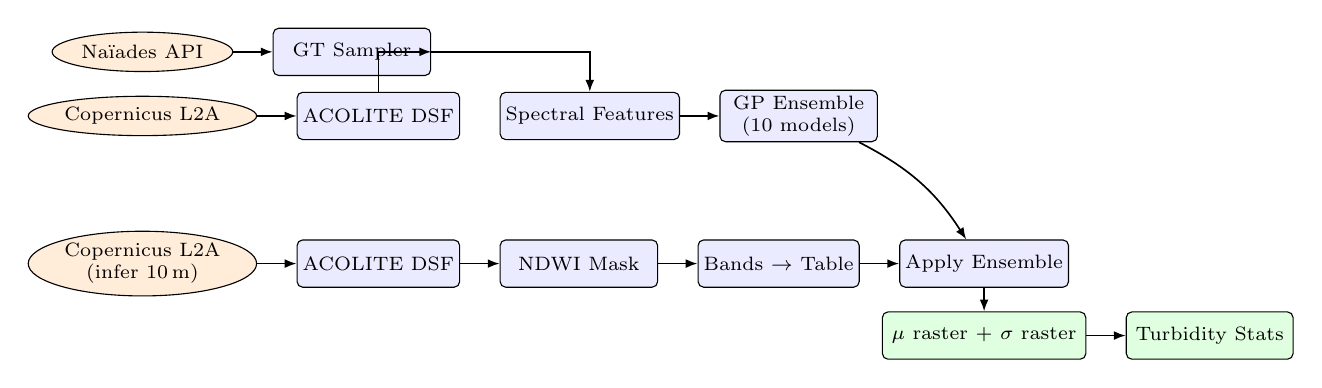
\begin{tikzpicture}[
    node distance=3mm and 5mm,
    every node/.style={font=\scriptsize, align=center},
    proc/.style={draw, rounded corners=2pt, fill=blue!8, minimum width=2.0cm, minimum height=0.6cm, inner sep=2pt},
    data/.style={draw, ellipse, fill=orange!15, minimum width=1.6cm, minimum height=0.5cm, inner sep=1pt},
    outbox/.style={draw, rounded corners=2pt, fill=green!12, minimum width=2.0cm, minimum height=0.6cm},
    arr/.style={-{Latex[length=1.5mm]}, semithick}
  ]

  \node[data] (api)   {Naïades API};
  \node[proc, right=of api] (gtsamp) {GT Sampler};
  \node[data, below=of api] (cop1) {Copernicus L2A};
  \node[proc, right=of cop1] (acol1) {ACOLITE DSF};
  \node[proc, right=of acol1] (sf1) {Spectral Features};
  \node[proc, right=of sf1] (gp) {GP Ensemble\\(10 models)};

  \node[data, below=12mm of cop1] (cop2) {Copernicus L2A\\(infer 10\,m)};
  \node[proc, right=of cop2] (acol2) {ACOLITE DSF};
  \node[proc, right=of acol2] (ndwi) {NDWI Mask};
  \node[proc, right=of ndwi] (bt) {Bands $\to$ Table};
  \node[proc, right=of bt] (apply) {Apply Ensemble};
  \node[outbox, below=of apply] (out1) {$\mu$ raster + $\sigma$ raster};
  \node[outbox, right=of out1] (stats) {Turbidity Stats};

  \draw[arr] (api) -- (gtsamp);
  \draw[arr] (cop1) -- (acol1);
  \draw[arr] (acol1) |- (gtsamp);
  \draw[arr] (gtsamp) -| (sf1);
  \draw[arr] (sf1) -- (gp);
  \draw[arr] (cop2) -- (acol2);
  \draw[arr] (acol2) -- (ndwi);
  \draw[arr] (ndwi) -- (bt);
  \draw[arr] (bt) -- (apply);
  \draw[arr] (gp)  to[bend left=15] (apply);
  \draw[arr] (apply) -- (out1);
  \draw[arr] (out1) -- (stats);
\end{tikzpicture}%
}
\caption{Pipeline graph as instantiated in VNStudio (schematic). Each box is a node; each arrow a typed connection (geotiff, dataframe, mask). The full graph is shipped as \texttt{public/templates/Machine Learning Course/gp\_ensemble\_uncertainty.vn}.}
\label{fig:pipeline}
\end{figure}

\begin{figure}[t]
\centering
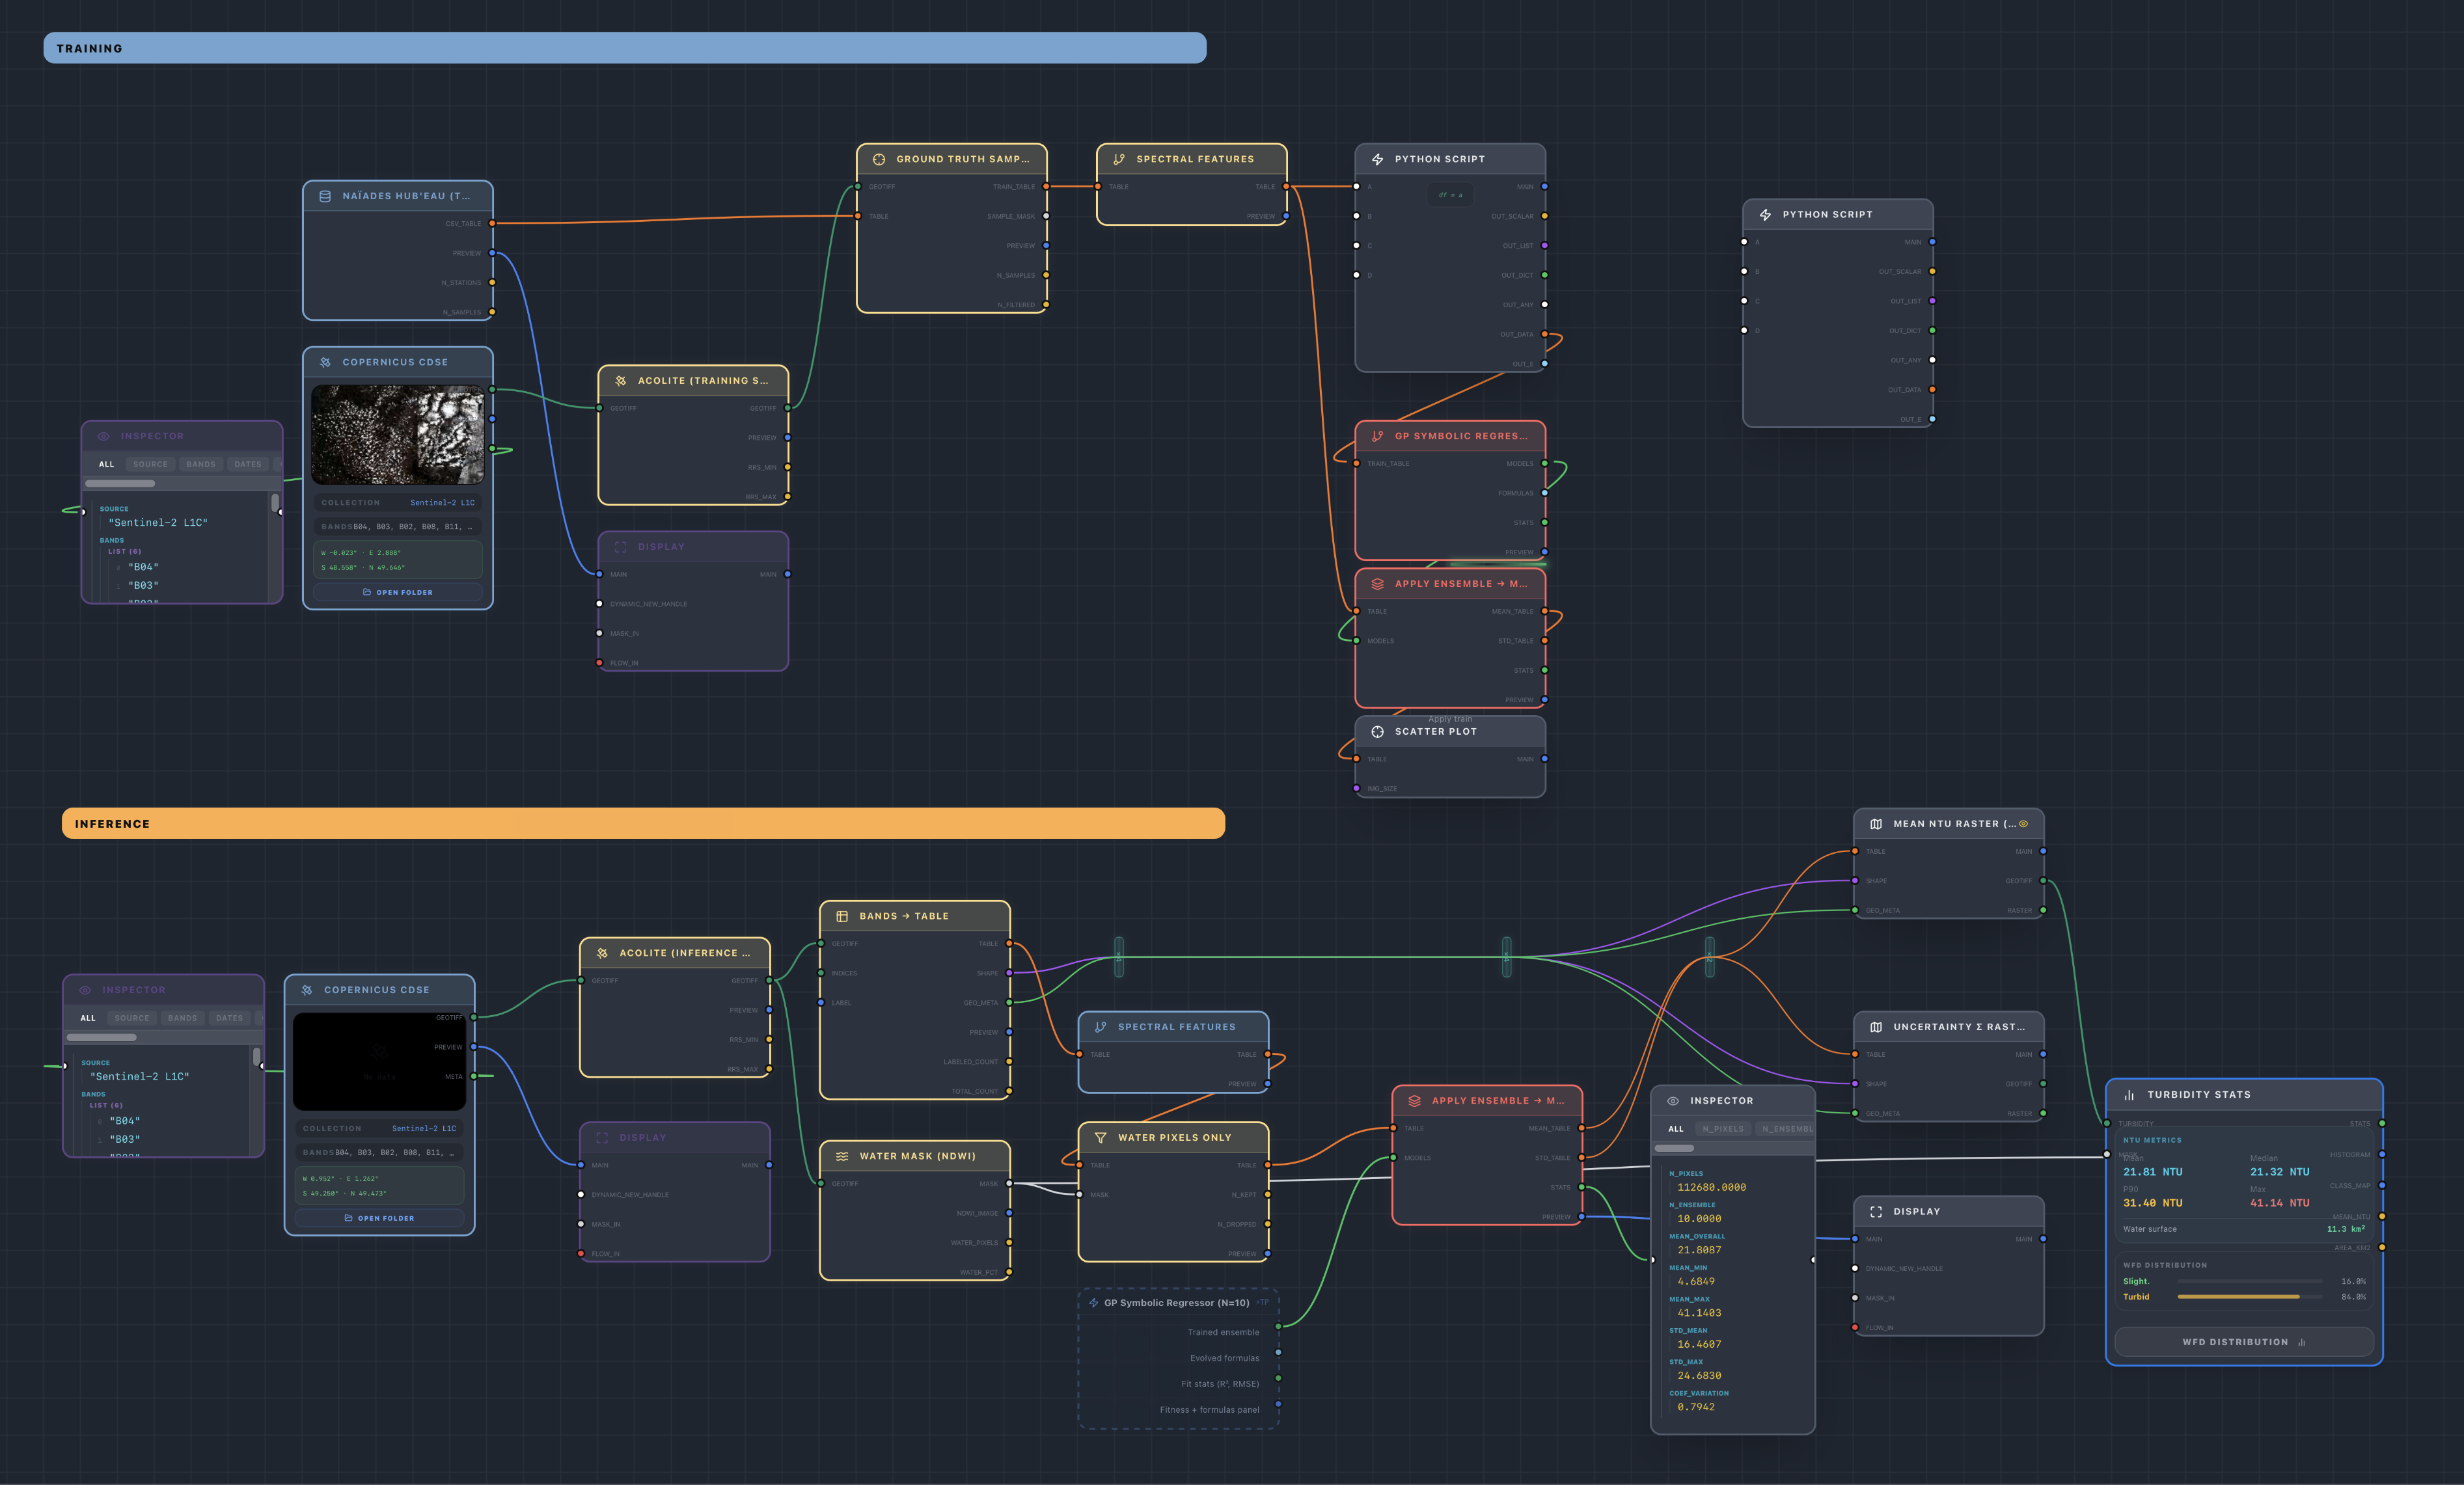
\includegraphics[width=\linewidth]{figs/pipeline_canvas.png}
\caption{Actual VNStudio canvas screenshot. Top swimlane: training branch (Naïades download $\to$ ACOLITE $\to$ Ground-Truth Sampler $\to$ Spectral Features $\to$ logic\_python rebalancer $\to$ GP Ensemble). Bottom swimlane: inference branch (Copernicus $\to$ ACOLITE $\to$ NDWI mask $\to$ Bands-to-Table $\to$ Apply Ensemble $\to$ Mean/Std rasters $\to$ Turbidity Stats). The entire experiment state lives in the JSON serialization of this canvas.}
\label{fig:canvas}
\end{figure}

The pipeline (Fig.~\ref{fig:pipeline}) splits into a \emph{training} branch (top) and an \emph{inference} branch (bottom), sharing a single GP ensemble. Sections~\ref{sec:atmcorr}--\ref{sec:stats} document each component and its parameters.

\subsection{Atmospheric correction (\texttt{geo\_acolite\_full}, DOS-1 mode)}
\label{sec:atmcorr}
Raw L2A reflectance still carries residual aerosol scattering and surface effects. We apply a fast Dark-Object Subtraction (DOS-1) variant on the L2A stream, configured with \texttt{band\_names = Blue,Green,Red,NIR,SWIR1,SWIR2} and \texttt{dsf\_aot\_estimate = dark\_spectrum}. Two implementation choices are non-obvious:
\begin{itemize}
    \item \textbf{Auto-scaling}: the test for ``raw DN vs. reflectance'' uses the 99th-percentile rather than the maximum, which would be dragged by a single saturated pixel and divide the entire scene by \num{10000}.
    \item \textbf{Dark-object selection}: the dark value is the 0.1$^{\text{th}}$ percentile of positive pixels, capped to discard cases where the 1$^{\text{st}}$ percentile coincides with the water signal. When $\textrm{dark} > 0.5 \times \textrm{median}$ the subtraction is skipped.
\end{itemize}
Output is Rrs $\in [0, 0.2]$ sr$^{-1}$, directly comparable to in-situ Rrs.

\subsection{Ground-truth sampling (\texttt{geo\_ground\_truth\_sampler})}
\label{sec:gtsamp}
The Naïades DataFrame is joined to the satellite raster through lat/lon $\to$ pixel mapping. Each station is sampled via a $5\times5$ \texttt{nanmean} window (smoothing sensor noise and co-registration error) and constrained by a $\pm$\SI{30}{\day} temporal window around the satellite date. Parameters:

\begin{center}
\small
\begin{tabular}{ll}
\toprule
Parameter & Value \\
\midrule
\texttt{lat\_col / lon\_col} & \texttt{lat / lon} \\
\texttt{target\_col} & \texttt{label} (NTU) \\
\texttt{band\_names} & Blue, Green, Red, NIR, SWIR1, SWIR2 \\
\texttt{target\_min / target\_max} & 0 / 500 NTU \\
\texttt{mask\_radius} & 3 px \\
\texttt{sample\_window} & 5 px (5$\times$5 nanmean) \\
\texttt{image\_date} & 2023-07-04 \\
\texttt{date\_window} & \SI{30}{\day} \\
\bottomrule
\end{tabular}
\end{center}

\subsection{Spectral feature engineering (\texttt{ml\_spectral\_features})}
\label{sec:specfeat}
Identical on the training and inference branches:
\begin{itemize}
    \item Ratios: \texttt{Red/Green}, \texttt{Blue/Green}, \texttt{Red/NIR}, \texttt{NIR/SWIR1}, \texttt{Red/SWIR1}
    \item Indices: $\textrm{NDTI} = (R-G)/(R+G)$, $\textrm{MNDWI} = (G - \textrm{SWIR1})/(G + \textrm{SWIR1})$
    \item Log transforms: $\log(\textrm{Red}), \log(\textrm{SWIR1})$
\end{itemize}
This expanded basis enlarges the symbolic search space without forcing a particular model shape.

\subsection{Symbolic regression ensemble (\texttt{ml\_symbolic\_regressor})}
\label{sec:gp}
We run \texttt{gplearn} 10 times with seeds $\{423, 424, \dots, 432\}$. Common parameters:

\begin{center}
\small
\begin{tabular}{ll}
\toprule
Parameter & Value \\
\midrule
\texttt{target\_column} & \texttt{label} \\
\texttt{n\_ensemble} & 10 \\
\texttt{population\_size} & \num{1000} \\
\texttt{generations} & 50 \\
\texttt{parsimony} & 0.001 \\
\texttt{test\_size} & 0.20 \\
\texttt{log\_transform} & True \\
\texttt{use\_log / use\_sqrt / use\_div} & True / True / True \\
\bottomrule
\end{tabular}
\end{center}

The function set is $\{+, -, \times, \div_{\textrm{protected}}, \sqrt{\,}, \log\}$. Training is performed in $\log(1+y)$ space, inverted at inference. Label distribution justifies the log transform: mean 13.02 NTU, $\sigma = 25.20$, range $[0.12, 240]$.

\subsection{Class-imbalance mitigation via stratified subsampling}
\label{sec:rebalance}
A direct GP run on the raw 563 matchups collapsed the ensemble to a near-constant predictor (predicted-vs-observed slope $\approx 0.02$): the parsimony penalty plus the heavy concentration of stations in the \emph{Clear} class (NTU $<5$, $\approx 80\%$ of training rows) makes a constant intercept a locally optimal expression. We therefore insert a \texttt{logic\_python} node in the training branch that retains only $30\%$ of the Clear-class rows (random subsample, seed 42) while keeping all rows with NTU $\geq 5$:

\begin{lstlisting}[language=Python]
clear_mask    = df['label'] < 5.0
df_clear_sub  = df[clear_mask].sample(frac=0.30, random_state=42)
df_turbid     = df[~clear_mask]
df_bal        = pd.concat([df_clear_sub, df_turbid], ignore_index=True)
\end{lstlisting}

This reduces the training set to $\approx 248$ rows but shifts the predicted-vs-observed slope from 0.02 to \textbf{0.26}, the regime reported in \S\ref{sec:results}. The choice of $30\%$ is empirical; sweeping this value is left as a sensitivity analysis (\S\ref{sec:future}).

\subsection{Water mask (\texttt{geo\_ndwi\_mask})}
NDWI = $(G - \mathrm{NIR}) / (G + \mathrm{NIR})$, thresholded at \texttt{0.1} and eroded by 2~px to remove mixed shoreline pixels.

\subsection{Inference and raster reconstruction}
The masked inference scene is unfolded to a per-pixel table (\texttt{geo\_bands\_to\_table}), passed through the trained ensemble (\texttt{ml\_ensemble\_apply}, \texttt{clip\_min=0}, \texttt{clip\_max=50}), then folded back to 2-D rasters using the original pixel indices (\texttt{geo\_table\_to\_raster}). Both $\mu$ and $\sigma$ maps inherit the CRS and affine transform of the inference scene.

\subsection{Statistics (\texttt{geo\_turbidity\_stats})}
\label{sec:stats}
WFD-style turbidity classes (\emph{Crystal}, \emph{Clear}, \emph{Slightly turbid}, \emph{Turbid}, \emph{Very turbid}, \emph{Extremely turbid}) are computed over the water mask. Parameters: \texttt{pixel\_m = 10}, \texttt{max\_ntu = 200}, \texttt{hist\_max = 100}.

% ─── 4. Results ──────────────────────────────────────────────────────────────
\section{Results}
\label{sec:results}

\subsection{Training set}
After the spatial and temporal joins, \textbf{563 satellite--station matchups} were assembled. Following the stratified subsampling of \S\ref{sec:rebalance} (retaining 30\% of NTU $<5$ stations), $\approx 248$ rows entered the GP search. Table~\ref{tab:bandstats} summarizes the input feature distribution on the full 563-row pool, before rebalancing; reflectances after DOS-1 lie within physically plausible bounds.

\begin{table}[h]
\centering
\caption{Training-set descriptive statistics (n = 563).}
\label{tab:bandstats}
\small
\begin{tabular}{lrrrr}
\toprule
Feature & Mean & Std & Min & Max \\
\midrule
Blue   & 0.054 & 0.057 & 0.002 & 0.200 \\
Green  & 0.049 & 0.052 & 0.003 & 0.200 \\
Red    & 0.070 & 0.051 & 0.026 & 0.200 \\
NIR    & 0.101 & 0.049 & 0.004 & 0.200 \\
SWIR1  & 0.080 & 0.048 & 0.002 & 0.200 \\
SWIR2  & 0.056 & 0.043 & 0.001 & 0.193 \\
\midrule
\textbf{label (NTU)} & 13.02 & 25.20 & 0.12 & 240.00 \\
\bottomrule
\end{tabular}
\end{table}

\subsection{Best-of-ensemble model}
The best individual across the 10 GP runs converges on the compact expression
\begin{equation}
    \mathrm{NTU} \approx \exp\!\Big(\,\underbrace{\tfrac{\mathrm{Blue}}{\mathrm{Red}}}_{\text{clarity ratio}} \;+\; \underbrace{\tfrac{\mathrm{NIR}}{\mathrm{SWIR1}}}_{\text{SPM proxy}} \;-\; \underbrace{\mathrm{Green}}_{\text{baseline}} \Big).
    \label{eq:bestmodel}
\end{equation}
(The $\exp$ wrapper inverts the log-target.) The three terms admit physical readings: $\text{Blue}/\text{Red}$ is the inverse Forel--Ule clarity index; $\text{NIR}/\text{SWIR1}$ captures residual reflectance in spectral regions where pure water absorbs strongly, so any signal indicates suspended particulate matter; the $-\mathrm{Green}$ term acts as a scene-brightness baseline. That this combination emerges from an unconstrained search --- without bands being labelled by their hydrological role --- is a tangible reproducibility check against the structural skeleton of the Nechad and Dogliotti models.

\subsection{Inference over the Rouen reach}
After NDWI masking, \num{112680} valid water pixels ($\approx \SI{11.3}{\kilo\metre\squared}$) entered inference. Ensemble statistics on the $\mu$-map:

\begin{table}[h]
\centering
\caption{Ensemble mean ($\mu$) statistics over the inference scene, before vs after the stratified-subsampling rebalancing of \S\ref{sec:rebalance}.}
\label{tab:mustats}
\small
\begin{tabular}{lrr}
\toprule
Metric & Baseline (NTU) & Rebalanced (NTU) \\
\midrule
Mean        & 5.07  & 21.81 \\
Median      & 3.53  & 21.32 \\
P90         & 6.21  & 31.40 \\
Maximum     & 45.27 & 41.14 \\
\bottomrule
\end{tabular}
\end{table}

Ensemble spread ($\sigma$) and dispersion:

\begin{center}
\small
\begin{tabular}{lr}
\toprule
Metric & Value \\
\midrule
Mean $\sigma$           & 3.78 NTU \\
Maximum $\sigma$        & 21.41 NTU \\
Coefficient of variation $\sigma/\mu$ & 0.87 \\
\bottomrule
\end{tabular}
\end{center}

WFD class distribution by water area (Table~\ref{tab:wfd}) confirms a low-flow summer regime: \SI{81}{\percent} of pixels classify as \emph{Clear} (1--5 NTU), with no \emph{Very turbid} or \emph{Extremely turbid} water.

\begin{table}[h]
\centering
\caption{WFD-class proportions over the \SI{11.3}{\kilo\metre\squared} masked water surface.}
\label{tab:wfd}
\small
\begin{tabular}{lrr}
\toprule
Class & NTU range & \% surface \\
\midrule
Crystal           & 0--1   & 4.7  \\
\textbf{Clear}    & 1--5   & \textbf{80.9} \\
Slightly turbid   & 5--15  & 9.5  \\
Turbid            & 15--50 & 5.0  \\
Very turbid       & 50--200& 0.0  \\
Extremely turbid  & $>$200 & 0.0  \\
\bottomrule
\end{tabular}
\end{table}

\subsection{Figures}

\begin{figure}[t]
\centering
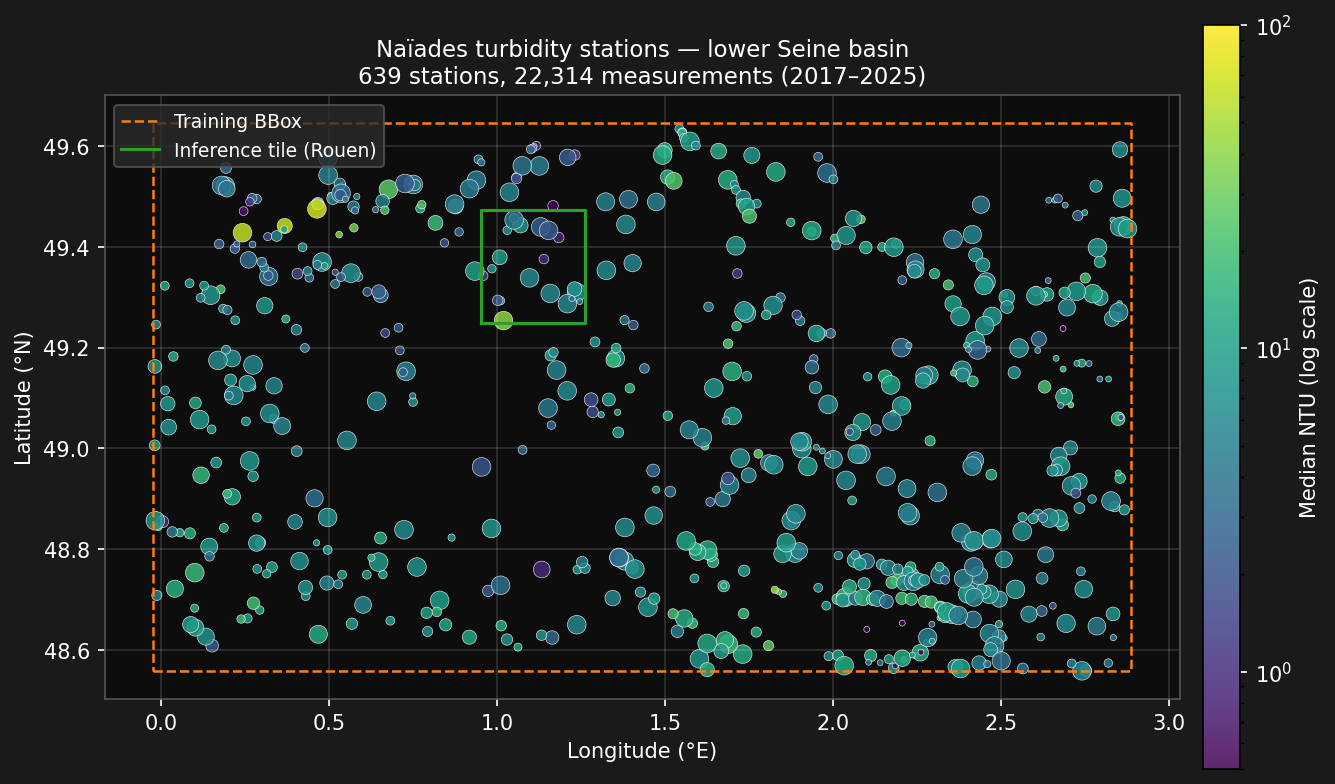
\includegraphics[width=0.75\linewidth]{figs/naiades_stations_map.png}
\caption{Naïades turbidity stations within the training bounding box (orange dashed, 2017--2025): 639 unique stations and 22{,}314 raw measurements, after filtering to NTU $\in [0, 500]$. Stations colored by median NTU (log scale); point size scales with the number of measurements. The green rectangle delineates the Rouen inference tile used in \S\ref{sec:results}.}
\label{fig:naiadesmap}
\end{figure}

\paragraph{Training-set fit.} A predicted-vs-observed regression on the rebalanced training set ($n \approx 248$, see \S\ref{sec:rebalance}) yields a positive but shallow slope of \textbf{0.26} (intercept 7.17 NTU): the model captures the direction of the NTU gradient yet systematically underestimates the upper tail, with observations above 100\,NTU predicted in the 30--65\,NTU range. The baseline run without stratified subsampling produces a near-constant predictor (slope 0.02), so the rebalancing recovers most of the signal even if the residual variance remains large.

\begin{figure}[t]
\centering
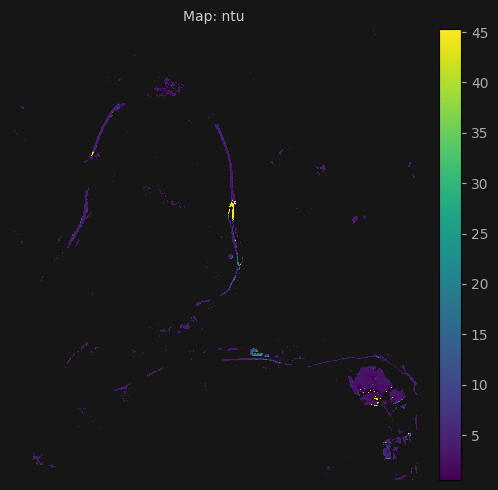
\includegraphics[width=0.85\linewidth]{figs/mu_raster.png}
\caption{Ensemble mean turbidity ($\mu$) over the Rouen reach (10\,m, 2023-07-04). Color scale: 0--50 NTU, NDWI water mask applied. The navigable channel is uniformly \emph{Clear} (1--5 NTU); turbid pockets concentrate along shorelines and side-channels.}
\label{fig:mumap}
\end{figure}

\begin{figure}[t]
\centering
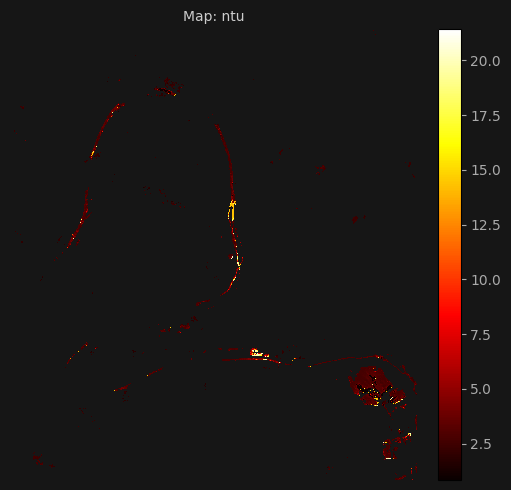
\includegraphics[width=0.85\linewidth]{figs/sigma_raster.png}
\caption{Ensemble standard deviation ($\sigma$) over the same scene. High-$\sigma$ pixels concentrate at land/water boundaries and near morphologically complex side-channels --- regions where individual GP models extrapolate differently.}
\label{fig:sigmap}
\end{figure}

\begin{figure}[t]
\centering
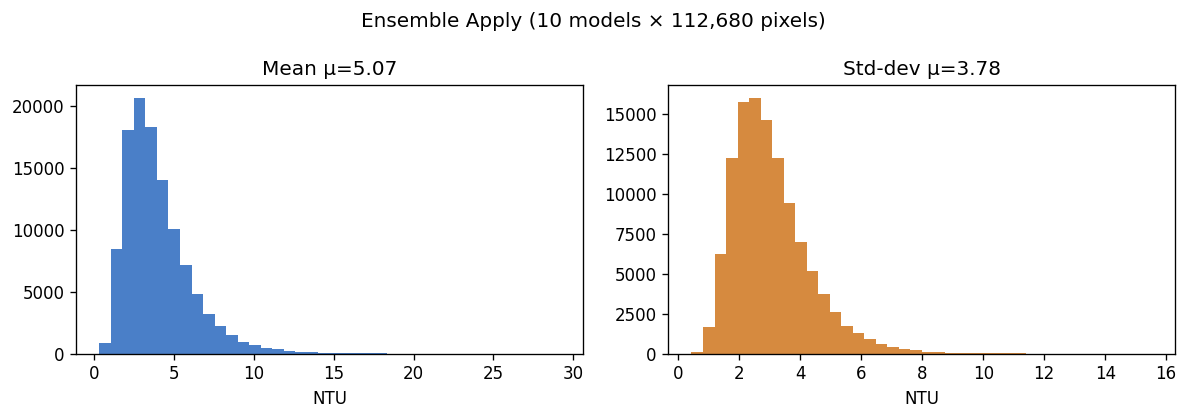
\includegraphics[width=0.85\linewidth]{figs/histograms.png}
\caption{Pixel-wise distribution of $\mu$ (left) and $\sigma$ (right) across the 112{,}680 water pixels of the inference scene.}
\label{fig:hist}
\end{figure}

\begin{figure}[t]
\centering
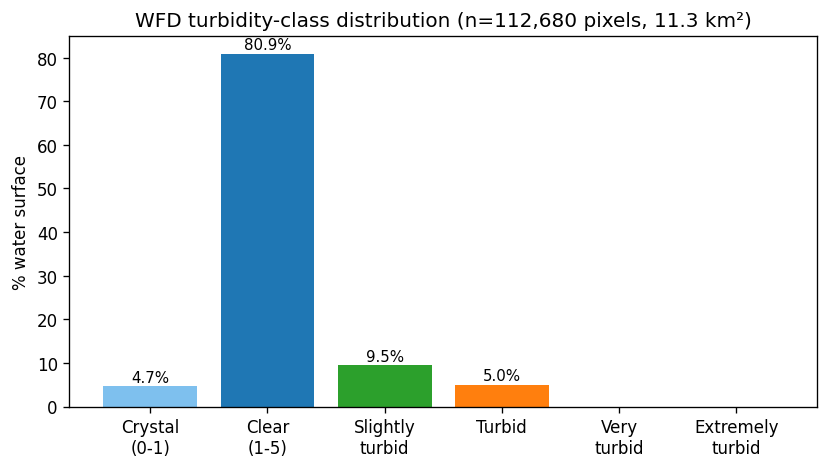
\includegraphics[width=0.7\linewidth]{figs/wfd_distribution.png}
\caption{WFD turbidity-class distribution: 81\% of the masked water surface is \emph{Clear} (1--5 NTU).}
\label{fig:wfd}
\end{figure}

% ─── 5. Discussion ───────────────────────────────────────────────────────────
\section{Discussion}
\label{sec:discussion}

\subsection{Why ensemble matters}
The coefficient of variation $\sigma/\mu \approx 0.87$ is the headline of the uncertainty analysis. Although the $\mu$-map (Fig.~\ref{fig:mumap}) appears spatially crisp, the ten ensemble members disagree by an amount comparable to the signal. Two factors plausibly drive this:
\begin{enumerate}
    \item \textbf{Residual training-set imbalance.} Even after the stratified subsampling of \S\ref{sec:rebalance}, the upper tail (NTU $>50$) is represented by fewer than 10 stations. Models extrapolate differently in that regime, producing the high-$\sigma$ pixels visible in Fig.~\ref{fig:hist} (right) and the systematic under-prediction of stations above 100 NTU reported in \S\ref{sec:results}.
    \item \textbf{Search-time stability.} GP rewards models that minimize training residuals but does not penalize input sensitivity. Adding a stability term across band perturbations would likely collapse the ensemble spread, at the cost of expressiveness.
\end{enumerate}
In practice, the $\mu$-map should be read as a class-level estimate (``Clear vs not-Clear''), and the $\sigma$-map should be consulted before any pixel-precise NTU claim. This is consistent with the proof-of-concept framing of \S\ref{sec:intro}.

\subsection{Rediscovery of physical structure}
Equation~\ref{eq:bestmodel} is structurally close to Nechad's red-band formula and Dogliotti's blended Red/NIR estimator: both rely on a clarity-sensitive visible ratio and an SPM-sensitive infrared term. That the GP search recovers this structure without supervision is, at minimum, a sanity check on the data preparation chain. It also suggests that fixed bio-optical models occupy a local optimum that purely empirical methods naturally drift toward when given enough freedom.

\subsection{Visual programming as a reproducibility primitive}
A common failure mode in remote-sensing experimentation is undocumented preprocessing: a Sentinel-2 scene is loaded, ``cleaned'', ``deglinted'', ``re-projected'', and by the time the regression is run the chain has accumulated ten implicit decisions that the manuscript does not record. A node-graph substrate forces every decision into a connector on a node, every parameter into a serializable field, and the whole graph into a single JSON file that can be re-opened and re-executed. We argue that this is not a UI niceness but a methodological prerequisite for the kind of multi-step, multi-source workflows that turbidity remote sensing entails.

% ─── 6. Limitations ──────────────────────────────────────────────────────────
\section{Limitations}
\label{sec:limit}
\begin{itemize}
    \item DOS-1 is a fast approximation of atmospheric correction. For publication-grade Rrs the \texttt{geo\_acolite\_full} node also exposes the full ACOLITE DSF entrypoint (\texttt{.SAFE} input), at $\approx$60\,s per scene.
    \item Naïades stations are biased toward monitored rivers; the model extrapolates poorly to estuarine plumes lying outside the training footprint.
    \item The $\pm\SI{30}{\day}$ temporal window is generous. Tightening to $\pm\SI{7}{\day}$ drops training to $\approx 100$ matchups but removes seasonal aliasing.
    \item GP \emph{best-of-ensemble} reporting hides multimodality: more than one expression family typically reaches near-equivalent test RMSE. Reporting only one obscures this.
    \item The predicted-vs-observed slope of 0.26 (\S\ref{sec:results}) shows the model captures direction but underestimates magnitude in the upper tail. Predictions saturate around 40--65\,NTU while observations extend to 240\,NTU.
\end{itemize}

% ─── 6.5. Future work ────────────────────────────────────────────────────────
\section{Future work}
\label{sec:future}

The proof-of-concept invites several concrete extensions, ordered roughly by expected effort:

\paragraph{Sample weighting in place of subsampling.}
The current rebalancing (\S\ref{sec:rebalance}) discards $\approx 70\%$ of the Clear-class rows. Passing a \texttt{sample\_weight} vector to \texttt{gplearn.SymbolicRegressor} (inverse class frequency, or a smooth density-based scheme) would preserve all training points and likely tighten the upper-tail predictions. This requires a small patch on \texttt{ml\_symbolic\_regressor} to accept a \texttt{weight\_col} parameter.

\paragraph{Tighter temporal matchups.}
The current $\pm\SI{30}{\day}$ window introduces seasonal aliasing. A second pass at $\pm\SI{7}{\day}$ on a multi-year, multi-tile dataset would test whether the underestimation is genuine model bias or a temporal mismatch.

\paragraph{Calibrated uncertainty.}
The ensemble $\sigma$ is uncalibrated --- there is no guarantee that $[\mu - 2\sigma, \mu + 2\sigma]$ covers $95\%$ of the true distribution. A standard conformal-prediction wrapper~\cite{angelopoulos2023}, trained on the held-out 20\% test split, would produce coverage-guaranteed intervals without retraining the GP.

\paragraph{Spatial transfer.}
The Rouen inference tile lies within the training footprint. Applying the model to a held-out basin (Loire, Rhône) would test whether the recovered symbolic structure generalises or whether basin-specific atmospheric / glint conditions drive the fit. The graph supports this directly: swap the \texttt{geo\_copernicus} BBOX and re-run inference, leaving the trained GP ensemble untouched.

\paragraph{Full ACOLITE DSF.}
The DOS-1 fast path used here approximates atmospheric correction. Switching the \texttt{geo\_acolite\_full} node to its \texttt{.SAFE} mode (\SI{60}{\second} per scene) would provide publication-grade Rrs and remove a confound from the comparison with published bio-optical models.

\paragraph{Multi-target GP.}
The same pipeline structure applies unchanged to chlorophyll-a, DOC, or total suspended solids, all available through the Hub'Eau API. A single graph could be parametrized over target column and bio-optical preset, providing a directly comparable benchmark suite across water-quality variables.

\paragraph{Expression-family analysis.}
Reporting only the best-of-ensemble formula hides the family of structurally distinct expressions that reach near-equivalent test RMSE. A clustering analysis of evolved formulas (by AST distance or by output-space similarity) would expose this multimodality and may surface alternative physical interpretations.

% ─── 7. Reproduction ─────────────────────────────────────────────────────────
\section{Reproduction recipe}
\label{sec:repro}

\begin{enumerate}
    \item Clone VNStudio:\\
        \texttt{git clone https://github.com/Nikos-Unilasalle/VisionNodes \&\& cd VisionNodes}
    \item Install:\\
        \texttt{npm install \&\& pip install -r engine/requirements.txt}
    \item Launch:\\
        \texttt{npm run studio}
    \item Open the template:\\
        \texttt{public/templates/Machine Learning Course/gp\_ensemble\_uncertainty.vn}
    \item Click \emph{Fetch} on the \textbf{Naïades} node (live Hub'Eau API).
    \item Click \emph{Fetch} on both \textbf{Copernicus} nodes (needs Copernicus credentials in \texttt{\textasciitilde/.config/copernicus.json}).
    \item Click \emph{Run} on both \textbf{ACOLITE} nodes ($<$5\,s each, DOS-1 mode).
    \item Click \emph{Train} on the \textbf{GP Ensemble} node ($\approx$30--60\,s for $10\times50\times1000$ GP search on a modern laptop).
    \item The $\mu$ / $\sigma$ rasters and the Turbidity Stats panel update automatically.
\end{enumerate}

% ─── Data & Code availability ────────────────────────────────────────────────
\section*{Data and code availability}
The complete pipeline (graph, plugins, and template) is available at \url{https://github.com/Nikos-Unilasalle/VisionNodes}. The training table and inference rasters used in this manuscript are deposited at \texttt{[Zenodo DOI placeholder]}.

% ─── Acknowledgements ────────────────────────────────────────────────────────
\section*{Acknowledgements}
We thank the Copernicus Data Space and the French Hub'Eau Naïades programme for open access to satellite and in-situ data, the \texttt{gplearn} maintainers for the symbolic regression engine, and the ACOLITE developers for the atmospheric-correction reference implementation.

% ─── Bibliography ────────────────────────────────────────────────────────────
\bibliographystyle{plain}
\bibliography{refs}

\end{document}
